This chapter provides an overview of the research related to the problem of route planning in food delivery. First, we describe the \emph{vehicle routing problem} and related \emph{pickup and delivery problem} along with their classification. Second, we focus on common solution methods from literature. Finally, we reveal some new methods that leverage machine learning and we mention some already available open-source solvers.

\section{Vehicle Routing Problem}

As adopted from Toth and Paolo (2015) \cite{toth2015vrp}, the family of \emph{vehicle routing problems} (VRP) can be defined as the following task:

\hfill\begin{minipage}{\dimexpr\textwidth-2cm}
    \vspace{.5cm}
    \textbf{Given} a set of \emph{transportation requests} and a \emph{fleet of vehicles},\\
    \textbf{determine} a set of \emph{vehicle routes} to perform all (or some) transportation requests with the given vehicle fleet \emph{at minimum cost}; in particular, decide which \emph{vehicle handles which requests and in which sequence} so that all vehicle routes can be \emph{feasibly} executed.
    \vspace{.1cm}
    % \xdef\tpd{\the\prevdepth}
\end{minipage}

	\begin{figure}[!ht]
		\centering
		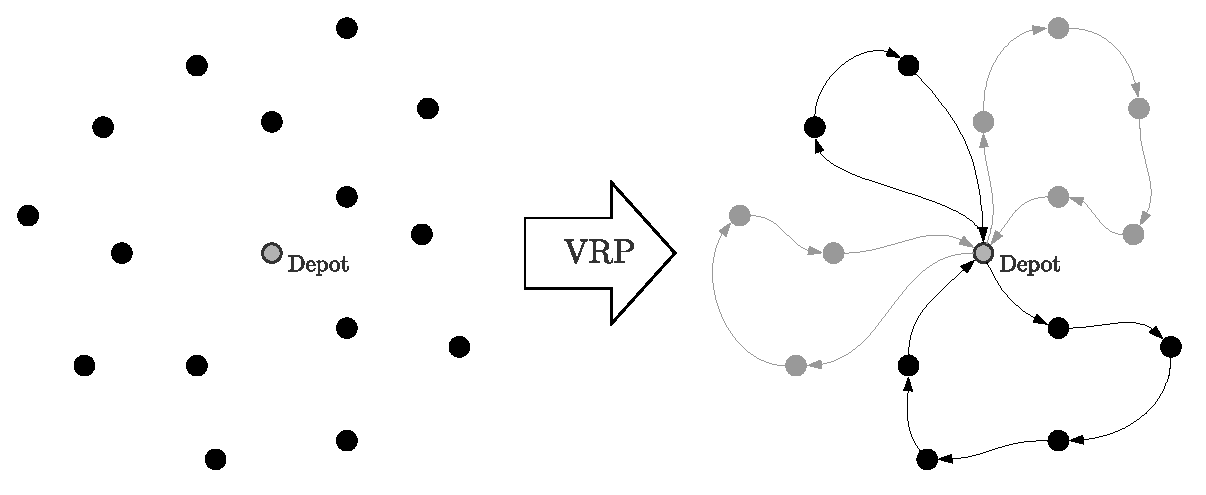
\includegraphics[width=0.8\textwidth]{figures/illustration.pdf}
		\caption[An intuitive view of the VRP instance and an example solution.]{An intuitive view of the VRP instance (left) and an example solution for four vehicles (right).}
		\label{fig:illustration}
	\end{figure}

In other words, the problem is concerned with finding the optimal routes to be followed by a fleet of vehicles to serve a set of customers \cite{golden2008the}. To better illustrate the problem, figure \ref{fig:illustration} shows an intuitive view of a VRP instance along with its example solution for four vehicles.

% Generally, in the VRP, the customers to be visited are modelled over graph nodes, whereas the problems where the requests are dispersed along the arcs are called \emph{arc routing problems} (ARP) \cite{corberan2014arc}.

The vehicle routing problem is one of the most studied problems in combinatorial optimization due to its relevance in industry \cite{golden2008the}. It belongs to the field of operations research applied to transportation problems. Figure \ref{fig:vrp-classes} shows the classification of VRP within operations research and puts in context the family of pickup and delivery problems that will be introduced later, and which is eminently important for this work.

	\begin{figure}[!ht]
		\centering
		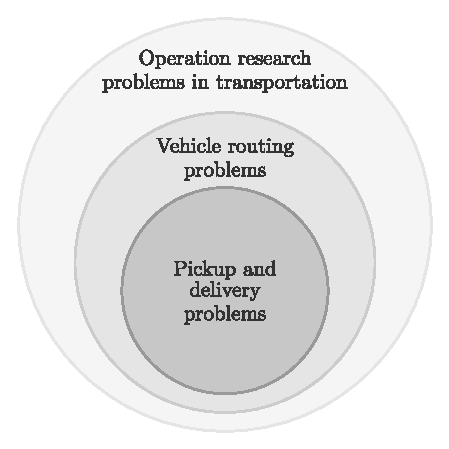
\includegraphics[width=0.6\textwidth]{figures/vrp-classes.pdf}
		\caption[The taxonomy of VRP and PDP within transportation-related operations research.]{VRP is one of many problems studied within transportation-related operations research. Pickup and delivery problems are a subclass of vehicle routing problems. The class of operations research contains many other problems apart from VRP, adopted from Ropke (2005)~\cite[p.~4~(modified)]{ropke-2005-phd}.}
		\label{fig:vrp-classes}
	\end{figure}

Numerous real-world applications have demonstrated the significance of computer-generated solutions of VRP in terms of global transportation costs \cite{toth2015vrp}. The success of optimization techniques can be attributed not only to the increasing computer power but also to recent research breakthroughs, the development of new mathematical models and to newly adopted approaches that leverage machine learning \cite{toth2015vrp, Falkner2020}. 

The VRP was first introduced in 1959 by Dantzig and Ramser \cite{1959} who came with the first mathematical model and an algorithmic approach using a simple matching-based heuristic. Since then, more than 80 years have passed and hundreds of models and algorithms have been proposed for different families of VRP as a result of a large variety of practical applications \cite{toth2015vrp}. This tendency has been enlarged by the burst of consumer delivery in the beginning of the century \cite{Falkner2020}. To show an example, the American logistics company UPS delivered around 11.5 million packages in 1993, compared to around 6.3 billion in 2020\footnote{\url{https://stories.ups.com/upsstories/us/en/about-us/global-presence/corporate-facts.html}} which counts for 24.7 million per single day.

Many variants of VRP have emerged over the years and the literature shows a clear trend towards the study of more complex variants to lower the gap between academic research and real-world applications. These problems imply constraints on various features the route must satisfy, such as vehicle capacity, pickup and drop-off times, or delivery sequence of operations. These classes of routing problems are often called \emph{rich VRPs} \cite{Mor2020}. These include \emph{capacitated VRP} (CVRP), in which each vehicle has predefined finite capacity that cannot be exceeded; the \emph{VRP with time windows} (VRPTW), where customers have to be served in predefined time intervals; the \emph{pickup and delivery problem} (PDP), where the goods (or people) to be transported have to be picked up at certain vertices as opposed to the depot; or the \emph{heterogenous fleet VRP} (HFVRP), in which vehicles may have different features, such as different capacities or can deliver only certain type of goods. Routing problems that involve transportation of people are referred to as \emph{dial-a-ride problem} (DARP) (or \emph{dial-a-flight problem} (DAFP) for air transportation) \cite{golden2008the, PILLAC20131}. These prevailing variants are detailed in the following sections and their taxonomy is clearly shown in figure \ref{fig:vrp-variants}. It is important to mention that these variants make just a fraction of the variants studied in the literature. Moreover, the distinction between the following variants of VRP is not always sharp and many combinations have been derived to more precisely represent real-world problems \cite{golden2008the, toth2015vrp, 2007-cordeau, cordeau-2007-7}.

	\begin{figure}[!ht]
		\centering
		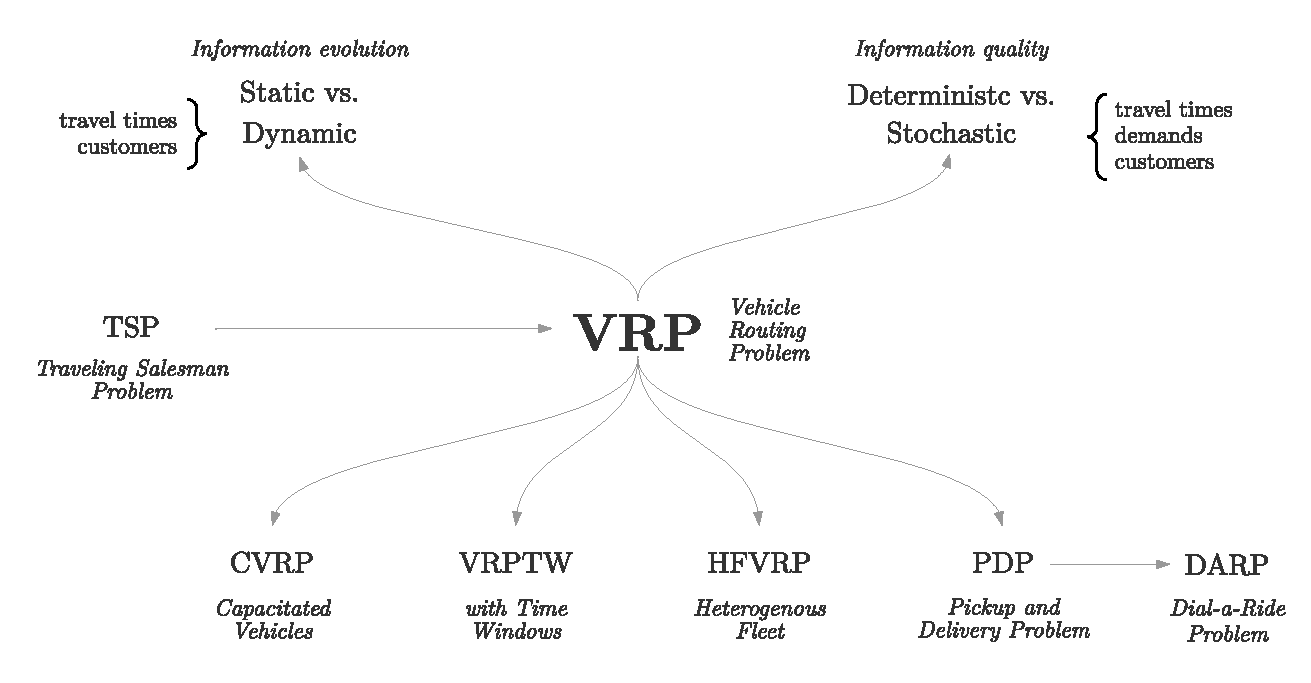
\includegraphics[width=1\textwidth]{figures/vrp-variants.pdf}
		\caption[Taxonomy of the VRP.]{Taxonomy of the VRP - the figure shows the prevailing variants of the VRP and common examples of static and dynamic elements, adopted from Bono (2020)~\cite[p.~26~(modified)]{Bono2020}.}
		\label{fig:vrp-variants}
	\end{figure}

\subsection{Capacitated Vehicle Routing Problem (CVRP)}

This variant of routing problems is the most studied in the literature, although it is mostly of academic relevance \cite{toth2015vrp}. In CVRP the requests correspond to the transportation of goods from a single depot to a set of customers. Each customer has a \emph{demand}, which is the amount to be delivered. The vehicle fleet is typically \emph{homogenous}, meaning that all vehicles have the same finite capacity and the same operational cost. Each vehicle starts at the depot, serves a disjunct set of customers, and returns to the depot \cite{toth2015vrp, cvrp-2019}.

\subsection{Vehicle Routing Problem with Time Windows (VRPTW)}

VRPTW is an extension of CVRP where the service at each customer location must occur within predefined time intervals, referred to as \emph{time windows}. There are two types of time windows commonly distinguished: soft and hard. Soft time windows can be violated carrying a penalty cost. In case of hard time windows, a driver must not arrive outside of the interval. The driver may arrive to the customer before the time window, however, the customer cannot be serviced until the time window starts. Arriving after the end of the time window is prohibited. Time windows can also be one-sided, i.e., defined as the earliest or the latest time of delivery \cite{wrptw, toth2015vrp, 2007-cordeau}.

\subsection{Heterogenous Fleet Vehicle Routing Problem (HFVRP)}

In this variant, vehicles are characterized by different features, such as different capacities, operational costs, or can only deliver a certain type of goods \cite{golden2008vrp, hvrp-2016, hvrp-2019}. There are two main branches of HFVRP regarding the obtainable fleet. In the \emph{unlimited} HFVRP, known as \emph{fleet size and mix VRP} (FSMVRP), the problem is to find the best fleet composition and routes, assuming that there is an unlimited number of vehicles of each type. In opposition, in the \emph{limited} HFVRP, known as \emph{heterogeneous VRP} (HVRP), the task is to find the optimal routes for the available fixed vehicle fleet \cite{hvrp-2019}. The cost of the solution usually depends on either the total distance traveled by all vehicles or the total enroute time. This problem is sometimes augmented by introducing time window constraints, making the HFVRP with time windows (HFVRPTW) \cite{hvrp-2016}.

In recent years, a relatively new variant related to HFVRP has emerged, called the \emph{green vehicle routing problem} (Green-VRP). The aim of Green-VRP is to minimize fuel consumption and to maximize the use of alternative fuel vehicles, such as electric vehicles, to reduce the impact on the environment. Usually, a heterogenous fleet of both classic and alternative fuel vehicles is considered during the planning process \cite{Asghari2021}.

\subsection{Pickup and Delivery Problem (PDP)}

Three known types of pickup and delivery problems are generally distinguished in the literature \cite{cordeau-2007-7, toth2015vrp}. First, the \emph{single-commodity} PDP, where a single type of good is either picked up or dropped-off at each of the customer location. An example of this problem might be transporting money from bank branch offices via an armored vehicle. Second, the \emph{two-commodity} PDP, in which two types of goods are being transported and each customer location may be used for both pickup and drop-off. This problem might occur, for example, in distribution of beverages, where the driver simultaneously delivers full bottles to the customer and collects the empty ones. A variant of the two-commodity PDP is a VRP with backhauls, where a pickup is only allowed when the vehicle is completely empty \cite{wrptw}. Finally, the \emph{n-commodity} PDP is where each type of good is associated with a single pickup location and a single drop-off location. A typical example of this problem can be a food delivery service \cite{cordeau-2007-7, 8541149, hvrp-2020}. In the literature, this problem is often referred to as \emph{vehicle routing problem with pickup and delivery} (VRPPD) \cite{cordeau-2007-7}.

From the implementation perspective, PDP setting introduces a new set of constraints. First, the constraints for the routes, such that the pickup and drop-off must be taken care of by the same vehicle. Second, the precedence constraint, i.e., the pickup happens before the drop-off \cite{Bono2020}.

A typical extension of PDP emanating from real-life usecases is the PDP with time windows (PDPTW). In this case, each pickup (drop-off) node is associated with a time interval, in which the driver can perform the pickup (drop-off) \cite{wrptw}.

\subsection{Dial-a-Ride Problem (DARP)}

The PDP also covers problems associated with people transportation. The major difference between transporting goods and people is the incorporation of customer satisfaction requirements. One of those problems is the so-called \emph{dial-a-ride problem} (DARP). This demand-responsive service is usually provided by a public authority to serve physically impaired people and elderly who may have difficulty using regular transport options \cite{toth2015vrp}. Unlike taxi and public transport services, passengers may share the ride with other passengers and, as a result, may deviate from the direct path from the pickup point to their destination \cite{darp-survey}. Some DARPs operate on a heterogenous fleet of vehicles, where different vehicles satisfy the different needs of physically impaired persons, for example, by being wheelchair accessible, some allow transfers from one vehicle to another \cite{belhaiza-2019, darp-survey}. The DARP implies that a set of customers make a request, which consists of origin and destination locations and imposes time window constraints for both pickup and drop-off. Additionally, customer inconvenience constraints are typically inflicted, such as maximum enroute time or maximum vehicle capacity \cite{toth2015vrp, belhaiza-2019}. There are three objectives of DARP that are often conflicting: maximizing the number of requests the fleet can serve, minimizing the overall operational cost, and minimizing customer inconvenience. A ratio between these objectives is sometimes achieved by first maximizing the number of requests that can be served by the available fleet of vehicles, and then minimizing the operational cost while acknowledging the inconvenience constraints \cite{cordeau-2007-7}.

Other people transportation problems related to DARP include \emph{dial-a-flight Problem} (DAFP) that concerns with air transportation \cite{PILLAC20131}, car pooling problem, which consists of finding groups of employees to share a car to work \cite{toth2015vrp}, Uber Pool service of an American company Uber \footnote{\url{https://www.uber.com/}} that combines taxi service with car pooling \cite{uber-pool}, or the \emph{school bus routing problem} (SBRP), where children in rural areas are picked up from the bus stop close to their homes and transported to their schools.


\subsection{Evolution and Quality of Information} \label{sec:evolution}

In contrast to the classical definition of VRP, real-world use cases often involve two important dimensions. The first one is \emph{evolution}, i.e., whether decisions are made a priori (referred to as \emph{static}) or the information changes in response to new information during the planning process, for instance, when new requests arrive or number of drivers changes (referred to as \emph{dynamic}). Second aspect is the \emph{quality of information}, i.e., whether the information is known with certainty before the start of planning (referred to as \emph{deterministic}) or there exists some amount of uncertainty when decisions are made (referred to as \emph{stochastic}). This categorization applies to VRP as well as DARP. \cite{PILLAC20131, darp-survey}

	\begin{figure}[!ht]
		\centering
		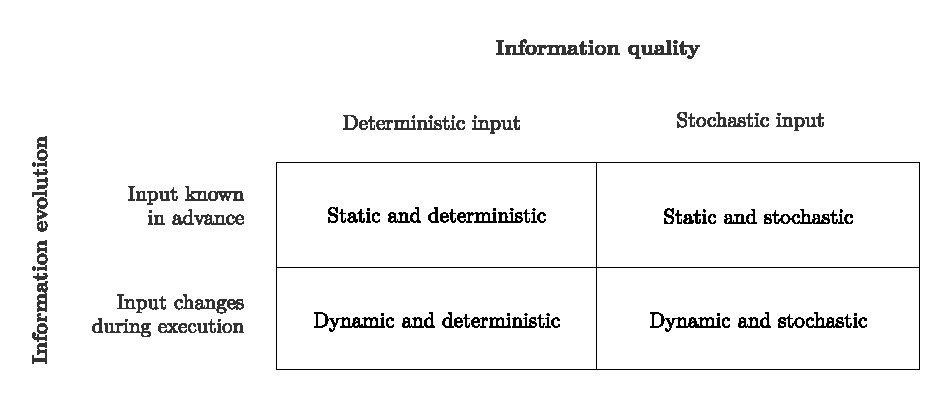
\includegraphics[width=0.9\textwidth]{figures/static-stochastic-table.pdf}
		\caption[Taxonomy of vehicle routing problems by information evolution and quality.]{Taxonomy of vehicle routing problems by information evolution and quality, adopted from Pillac et al. (2013)~\cite[p.~2~(modified)]{PILLAC20131}.}
		\label{fig:static-stochastic-table}
	\end{figure}

Based on these dimensions, four categories of routing problems are identified and are shown in figure \ref{fig:static-stochastic-table}. In \emph{static and deterministic} problem, all information is known before the decisions are made and does not change during the execution of planning. It is sometimes referred to as \emph{clasical} problem \cite{PILLAC20131}. \emph{Static and stochastic} problems are the ones where some information is unknown or uncertain at the time of decision, but information about the uncertainty may be known, i.e., in the form of an available range or probability distribution. In addition, routes are planned a priori and only slight changes are allowed during the execution, for example, adding a new node at the end of the plan or skipping a customer. These types of problems do not require any additional technological support. Most of the research in this field is focused on stochastic customers, stochastic time windows, and stochastic demands \cite{GENDREAU19963, 2007-cordeau, stoch-demands}.

\emph{Dynamic and deterministic} problems work with some part of the input that is unknown and revealed dynamically during the execution of planning. Thus, the routes for the drivers need to be constantly updated, which requires additional technological support for providing additional information to the planner, such as the location of the drivers using their mobile phones with GPS \cite{2007-cordeau, online-routing-2007}. Some authors also call these problems \emph{real-time} or \emph{online} \cite{online-routing-2007}. \emph{Dynamic and stochastic} problems are similar to the previous type, but additionally, stochastic knowledge about the dynamically revealed information is available.



\section{Solution Methods}

The approaches to solve vehicle routing problems are generally divided into two categories: exact and heuristic. The exact methods guarantee to find the optimal solution when sufficient resources are provided. However, until now, only small instances of VRP problems involving only up to tens of customers can be solved optimally due to high computational complexity \cite{toth2015vrp, Peng2020}. Indeed, VRP belongs to the class of NP-hard problems \cite{time-complexity-vrp}. Moreover, according to Savelsbergh (1985) \cite{Savelsbergh1985}, even finding a feasible solution for the VRPTW is itself an NP-complete problem. Nonetheless, some amply constrained problems with reasonable-sized instances can be solved to optimality via mathematical programming techniques \cite{2007-cordeau}, which are covered in section~\ref{sec:exact-methods}.

In real-life problems, exact methods are oftentimes insufficient as large instances need to be solved in a relatively short time. Therefore, heuristic approaches are required to tackle real-world problems. With the trade-off between the computation time and optimality, heuristic algorithms are able to find solutions of relatively good quality within acceptable computational time even for large instances \cite{Peng2020}. In addition, heuristic algorithms offer a decent amount of flexibility which allows to target different problem settings that vary in constraints and objectives \cite{toth2015vrp}. However, heuristic algorithms lack the theoretical guarantee regarding the quality of produced solution. Observations about solution quality can only be made empirically based on experiments \cite{ropke-2005-phd, Peng2020}.

A class of heuristic algorithms that has gained attraction over the last years is \emph{metaheuristics}. They provide a general framework for heuristics applicable to many problem variants and they often generate solutions of very high quality \cite{ropke-2005-phd}. In fact, metaheuristics are capable of yielding solutions within seconds whose values lie within one percent from the best known values \cite{toth2015vrp}. Heuristic algorithms are further described in section \ref{sec:heuristics}.

Another special class of heuristics that should be mentioned are \emph{approximation algorithms}. These methods provide both a solution and an error guarantee. For instance, they could guarantee that the obtained solution is at most $k$ times worse than the best obtainable solution \cite{vazirani2001approximation}.

% However, approximation algorithms are not the focus of this work and will not be covered in more detail.

The following sections provide an overview of both exact and heuristic methods for solving the VRP. More emphasis is being put on metaheuristic approaches as they are currently the state-of-the-art solution for most real-world VRP problems \cite{toth2015vrp}.

\subsection{Exact Methods} \label{sec:exact-methods}

For many real-world problems, the solution space is so large that even if we had a computer that could evaluate the cost of a trillion solutions per second, and we had started it right after the big bang, around 14 billion years ago, it would not have evaluated all feasible solutions by today. Therefore, exact algorithms need to use other methods rather than simple enumeration \cite{ropke-2005-phd}. This section lists a few most popular exact methods. For a detailed description and an extensive survey, we refer the readers to Toth and Paolo (2015) \cite{toth2015vrp} and Ho at al. (2018) \cite{darp-survey}.

The CVRP is the oldest and the most basic variant of the VRP, hence the first exact methods were developed mostly for the CVRP and later extended to be used with other VRP variants. The CVRP is an extension of the known \emph{travelling salesman problem} (TSP), where the task is to find a Hamiltonian circuit with minimum cost while visiting each node exactly once \cite{toth2015vrp}. The TSP was first formulated in 1930, around 30 years earlier than the VRP \cite{tspsurvey, 1959}. Therefore, the foundation of many exact algorithms for the CVRP builds on the thorough work done for the exact solution of the TSP \cite{toth2015vrp}. However, as it turns out, the CVRP is significantly harder to solve in practice compared to the TSP. The best exact methods for the CVRP are rarely able to solve instances with over a hundred customers, whereas the TSP instances with thousands of nodes are now routinely solved to optimality \cite{2007-cordeau}.

Exact methods directly address the problem using integer linear programming. The objective is to find a binary assignment for decision variables, modelling connections between vehicles and nodes, while minimizing the objective value \cite{Bono2020}. The early methods to solve the CVRP were mainly direct tree search algorithms based on branch-and-bound (B\&B) \cite{toth2015vrp}. Algorithm \ref{alg:bab} shows a main loop of branch-and-bound.

The computational complexity of the B\&B can be exponential in the worst case \cite{darp-survey}, thus some relaxations need to be employed to speedup the search. The combinatorial relaxations used in the branch-and-bound algorithms were adopted from what was earlier proposed for the TSP \cite{tspalg} and later extended by better relaxation techniques based on Lagrangian relaxations and the additive approach. These methods were able to solve instances with lower tens of customers to optimality \cite{toth2015vrp}. Later, branch-and-cut algorithms exploited cutting planes to tighten the linear programming relaxations, which led to a higher chance of finding integer solutions, and provided stronger bounds for optimality verification. In contrast, branch-and-price algorithms focused on column generation rather than generating cuts, which allowed to solve larger mixed-integer programs while still guaranteeing the convergence to global optimum \cite{toth2015vrp, darp-survey}. Current best algorithms for the CVRP belong to the branch-and-price-and-cut family, which combines cuts and column generation, and are much more effective than each of those techniques alone \cite{Fukasawa2006}.


\begin{algorithm}[!ht]
\SetAlgoLined
 currentBest, upperBound $\leftarrow$ FindInitialSolution(problem)\;
 add problem to queue\;
 \While{queue is not empty}{
  problem $\leftarrow$ pop item from queue\;
  \For{subProblem in branch}{
    \If{CanSolve(subProblem)}{
     candidate, cost $\leftarrow$ Solve(subProblem)\;
     \If{cost $\leq$ upperBound}{
      currentBest, upperBound $\leftarrow$ candidate, cost\;
     }
    }
    \ElseIf{LowerBound(subProblem) $\leq$ upperBound} {
      add subProblem to queue\;
    }
  }
 }
 \caption{Branch-and-Bound, adopted from Bono (2020)~\cite[p.~34~(modified)]{Bono2020}.}
 \label{alg:bab}
\end{algorithm}

Branch-and-price is largely used for solving a variety of routing problems and is not constrained to only the CVRP. For the VRPTW, this approach was first used by Desrochers, Desrosiers, and Solomon (1992) \cite{Desrochers1992}. The branch-and-price-and-cut algorithm was also later applied to VRPTW by Kohl et al. (1999) \cite{Kohl1999}.

Similarly, for the pickup and delivery problems, Lu and Dessouky (2004) \cite{branchAndCut} and later Ropke et al. (2007) \cite{branchAndCut2} have used the branch-and-cut algorithms for the PDPTW. Their approach was able to solve instances of up to 75 customers to optimality. The branch-and-cut-and-price algorithm by Ropke et al. (2009) \cite{branchCutPrice} was able to solve some highly constrained instances of PDPTW of up to 500 customers. In the DARP setting, most of the exact methods are also built upon the concept of branch-and-bound \cite{darp-survey}. For multiple vehicles, methods based on branch-and-price seem to be the most promising in the current state of the art. Still, most PDP instances remain much harder to solve than the same-size instances of classical VRP. This is predominantly caused by the precedence constraints, which generally lead to poor linear programming relaxations \cite{toth2015vrp}.

The main advantage of using the exact methods is that the optimality of the solution is guaranteed. This is particularly important for static problems. Therefore, the majority of the research in exact algorithms focuses on static and deterministic problems. Computational times of several hours are acceptable for problems, where the information is provided in advance and no changes are expected. Even if the optimal solution cannot be retrieved by the exact algorithm, the planner is able to measure the optimality gap, aka how far the solution can be from the optimum \cite{darp-survey}.


\subsection{Heuristic Methods} \label{sec:heuristics}

When problems are not manageable by exact methods, for instance, due to unacceptable computational time or memory issues, heuristics are essential to provide high-quality solutions \cite{darp-survey}. The field of VRP heuristics is so rich nowadays that it would be an unimaginable task to describe or even list all of them in this section. Instead, we summarize the most prevailing methods that are still being actively used and present some new and promising techniques.

The progression of heuristic approaches for VRP in the last decade has been primarily in the context of metaheuristics. What best describes this progression is the hybridization of both concepts and scope. First, there has been an emergence of new heuristics that combine several concepts in terms of search principles that have been initially developed individually, such as genetic algorithms, tabu search, large neighborhood search, or simulated annealing. In addition, other strategies and techniques have found their place in the most popular methods. These include exotic large neighborhoods, exact mathematical techniques, decomposition, and cooperation schemes, to name a few. Second, the hybridization of scope in heuristics means that they offer a decent amount of flexibility which allows to target different problem variants with various constraints and objectives without any extensive structural changes \cite{toth2015vrp}.

The following two sections summarize some relevant results regarding constructive heuristics and metaheuristics. We also take a brief look at the latest advancements in machine learning methods for VRP.

\customsubsubsection{Constructive Heuristics}

Constructive heuristics are frequently utilized to quickly create an initial feasible solution. Although metaheuristics are more effective, constructive heuristics are employed in various dynamic problems that require a feasible solution within milliseconds \cite{Markovic2015, Wong2014}, or to evaluate various operational policies \cite{Wong2014}. In many cases, solutions obtained via constructive heuristics are used to provide an initial solution for more complex methods \cite{Masmoudi2016, Braekers2014}. However, many metaheuristics are so robust that they can be initialized with any random solution, which does not even need to be feasible, and still produce high-quality results \cite{toth2015vrp}.

Most constructive heuristics are inspired from the greedy insertion heuristic introduced by Jaw et al. (1986) \cite{Jaw1986}, who was the first to adapt the traditional insertion algorithm to DARP with time windows and multiple vehicles. The algorithm selects the requests sorted by the earliest pickup time and inserts the request into the cheapest feasible position in the existing routes. Alternatively, it adds a new vehicle if no feasible position is found.

Lu and Dessouky (2006) \cite{insertionHeuristics} proposed an insertion-based heuristic for the PDPTW, which regarded the deviations from time windows and an increase in travel time. The results show that the heuristic outperforms several decent methods on standard benchmarking problems. A similar approach was taken by Fielder et al. (2018) \cite{fiedler} in a dial-a-ride setting.

\customsubsubsection{Metaheuristics}

Metaheuristics for the VRP can be loosely classified into two categories: local search methods and population-based methods. However, the frontiers between these methods have become increasingly fuzzy in recent years and many hybrid methods have emerged. They will also be discussed in this section.

Local search algorithms start from an initial solution $x_0$ and at each iteration $t$, they move from the current solution $x_t$ to another solution $x_{t+1}$ in its neighborhood $N(x_t)$. The neighbors are retrieved by applying operators, which make minor modifications of the original solution. If any neighbor yields a better performance, i.e., the cost $c(x_{t+1})$ is lower than $c(x_t)$, it becomes the new candidate solution. However, local search algorithms usually allow worsening of the solutions, such that the cost $c(x_{t+1})$ does not always have to be lower than $c(x_t)$, to better explore the solution space and escape the local optimum. As a result, certain mechanisms must be put in place to avoid cycling \cite{Bono2020, toth2015vrp}. Algorithm \ref{alg:local-search} shows a common main loop of local search algorithms.

\begin{algorithm}[!ht]
\SetAlgoLined
 candidate $\leftarrow$ FindInitialSolution()\;
 best $\leftarrow$ candidate\;
 \While{stopping criterion is not met}{
    \If{IsValid(candidate) and Cost(candidate) $<$ Cost(best) }{
     best $\leftarrow$ candidate\;
    }
    neighbor $\leftarrow$ FindBestNeighbor(candidate)\;
    \If{Cost(neighbor) $<$ Cost(candidate) or AllowWorse(neighbor)} {
      candidate $\leftarrow$ neighbor\;
    }
 }
 \caption{Local Search, adopted from Bono (2020)~\cite[p.~36~(modified)]{Bono2020}.}
 \label{alg:local-search}
\end{algorithm}

\customparagraph{Tabu Search}

One of the local search algorithms is \emph{tabu search}. It moves from a solution $x_t$ to the best non-tabu solution $x_{t+1}$ in its neighborhood $N(x_t)$. To avoid cycling, it keeps a list of previous candidate solutions that are declared \emph{tabu}, or forbidden, to the completion of the algorithm, or for a certain number of iterations \cite{toth2015vrp}.

Tens of different implementations of tabu search have been proposed over the years. One of the first metaheuristics for PDPTW was an algorithm proposed by Nanry and Barnes (2000) \cite{nanryBarnes}. They developed the tabu search with three operators: moving a pickup-drop pair into another plan, switching two pickup-drop pairs between plans and moving individual nodes within the plan. Cordeau and Laporte (2003) \cite{Cordeau2003} were among the first to use the tabu search for the DARP with satisfactory results. Moreover, Zachariadis and Kiranoudis (2010) \cite{Zachariadis2010} showed that tabu search can perform very well even on large-scale instances.

\customparagraph{Simulated Annealing}

\emph{Simulated annealing}, another well-known local search operator uses a technique inspired by the physical annealing process. The solution $x_{t+1}$ is usually randomly selected from the neighborhood $N(x_t)$. To avoid being stuck in a local optimum, worse or nonimproving solutions are accepted with a given probability \cite{Bono2020}. One known implementation of this algorithm for the VRP is that of Osman (1993) \cite{Osman1993}.

One of the recent studies conducted by Braekers et al. (2014) \cite{Braekers2014} proposed a highly effective deterministic variant of simulated annealing, named \emph{deterministic annealing}. In this study, nonimproving solutions are accepted while the deterioration of the objective value is lower than a deterministic threshold. Braekers et al. used more complex operators and, in addition, a restart strategy to escape unattractive regions of the search space.

\customparagraph{Variable Neighborhood Search}

Both the tabu search and simulated annealing work well as standalone algorithms, but are widely used in combination with local search heuristics, such as \emph{variable neighborhood search} \cite{Gendreau2001, Schneider2014}. This algorithm was first proposed by Mladenovi{\' c} and Hansen (1997) \cite{Mladenovic1997}. It works with several neighborhoods ($N_1,\ldots,N_p$) that are systematically changed in the descent and preturbation phases of the local search. The algorithm starts from an initial solution $x_0$ and iteratively applies these neighborhoods until no improvement is achievable. After the last applied neighborhood, the cycle restarts. The algorithm usually finishes after a defined number of cycles or, as introduced by Li and Lim (2003) \cite{liLim}, when the solution is no longer improving.

Kytöjoki et al. (2007) \cite{KYTOJOKI2007} were among the first who successfully applied variable neighborhood search to solve the VRP. Two years later, Parragh et al. (2009) \cite{Parragh2009} proposed a variable neighborhood search for the DARP. Thanks to the great results, more researchers have adapted the algorithm to other DARP usecases in recent years \cite{SCHILDE2011, SCHILDE2014, MUELAS2013, MUELAS2015, Detti2017}. Variable neighborhood search proved to be able to obtain high-quality solutions even for large-scale VRP instances of up to 20,000 customers \cite{toth2015vrp}.

\customparagraph{(Adaptive) Large Neighborhood Search}

One of the most successful metaheuristics for a wide variety of routing problems is \emph{large neighborhood search} \cite{Gschwind2016}, first introduced by Shaw (1997) \cite{Shaw1997}. At each iteration, part of the current solution is destroyed (e.g., $k$ requests are removed) by applying one or more removal operators and rebuilt again into a new complete solution using one or more insertion operators \cite{darp-survey}. The modifications of solutions are commonly bigger than those of previously described heuristics. In an adaptive extension of this algorithm, called \emph{adaptive large neighborhood search}, the removal and insertion operators are selected based on their past performance during the search, usually by employing a roulette wheel selection process with an adaptive weight adjusting mechanism \cite{Azi2014, Gschwind2016, Masmoudi2020}.

Ropke and Pisinger (2006) \cite{Ropke2006} used the adaptive large neighborhood search heuristic to solve the PDP with time windows. Their algorithm used removal and insertion operators already existing in the literature, including the removal operator by Shaw (1997) \cite{Shaw1997}, and an acceptance criterion for new solutions known from simulated annealing. The algorithm by Ropke and Pisinger has proven to be powerful and has served as a building block for many further studies in complicated routing problems, particularly PDP and DARP \cite{Gschwind2016, Braekers2016, Masmoudi2016, Belhaiza2017, Drexl2018, Belhaiza2019, Masmoudi2020, Wang2020, Cauchi2020, Malheiros2021}. Gschwind and Drexl (2016) \cite{Gschwind2016} adopted the algorithm from Ropke and Pisinger and added three more removal operators. They also demonstrated how to test a new solution for feasibility in an amortized constant time. Their version of the adaptive large neighborhood search produced better solutions on standard DARP instances compared to the vast majority of other algorithms, except for the hybrid genetic algorithm by Masmoudi et al. (2017) \cite{Masmoudi2017}.

\vspace{0.5cm}

The other well-known category of metaheuristics are population-based methods, which are inspired by natural processes, such as the evolution of species or the behavior of insects. All successful population-based heuristics rely on local search methods to drive the search towards promising areas and to avoid local optima. As a result, the majority of population-based algorithms are naturally hybrid \cite{toth2015vrp}.

\customparagraph{Ant Colony Optimization}

This metaheuristic has also proven practical for many routing problems. It is inspired by the pheromone mechanism used by ants for coordination. Each ant simulates a solution by traversing the graph along its edges and accumulates pheromons along the edges it traversed. In each iteration, the ants select the edges with a probability proportional to the pheromon value. The pheromon evaporates after a given number of iterations, so the most promising edges remain at the end \cite{Bono2020, Solnon2010}. The algorithm by Reimann et al. (2004) \cite{Reimann2004} was one of the most successful.

Ant colony optimization algorithm is particularly interesting in dynamic and stochastic settings. When new information is received, such as a new request arrives, or some delays occur, the algorithm uses the pheromone trails from previous iterations. This relies on the assumption that the new information does not disrupt the current solution too much and that some patterns can still be exploited \cite{Schyns2015, Bono2020}.

\customparagraph{Genetic Algorithms}

\emph{Genetic algorithms} are population-based methods that are inspired by the evolution of species. These algorithms usually work with not a single solution, but rather a population of solutions, called \emph{individuals}. At each iteration, the individuals with better fitness are selected with higher probability to be parents. New individuals are created by applying the crossover and mutation operators to the parents and added to the population, while some other individuals are replaced \cite{Bono2020, darp-survey}.

The first successful application of genetic algorithms to solve the VRP is that of Prins (2004) \cite{Prins2004}. Prins combined the genetic operators, selection and crossover with a local search method to replace the classic random mutation operator. Other researchers successfully applied genetic algorithms for numerous VRP variants, for example, Masmoudi et al. (2017) \cite{Masmoudi2017} proposed a hybrid genetic algorithm to tackle the DARP with excellent results, even outperforming in terms of quality of solution, many large neighborhood search algorithms that are usually better performing on larger instances \cite{darp-survey}.

\customsubsubsection{Hybrid Algorithms}

Combining metaheuristics with other metaheuristics or exact methods is a growing trend that has proven successful. Indeed, many state-of-the-art algorithms for combinatorial optimization problems are hybrid algorithms.

In the literature, hybrids of metaheuristics are the most prevalent \cite{darp-survey}. They usually come in two forms. First, each metaheuristic is executed sequentially, for example, in a study by Parragh et al. (2009) \cite{Parragh2009}, where several algorithms are applied to the best solutions obtained from the previous algorithms. The other option is that one metaheuristic is executed in another metaheuristic. A popular approach is to embed local search methods into population-based heuristics, which takes advantage of combining the exploration ability of population-based heuristics with the exploitation ability of local search methods. Examples of this approach are the studies by Masmoudi et al. (2016 and 2017) \cite{Masmoudi2016, Masmoudi2017}.

Hybrids of metaheuristics with exact methods are also employed. They are obtained by either embedding a metaheuristic to the mathematical or constraint programming approach or vice versa. An example could be a research conducted by Parragh and Schmid (2013) \cite{Parragh2013}. They combined a column generation approach with a variable neighborhood search. To improve the obtained solutions, a large neighborhood search was employed. Another example could be the study by Gschwind and Drexl (2016) \cite{Gschwind2016} in which dynamic programming
is used within a large neighborhood search.

\customsubsubsection{Leveraging Machine Learning} \label{sec:machine-learning}

Designing a good heuristic algorithm is difficult as it requires expert knowledge of the problem and often involves the incorporation of custom features or constraints. Several alternative approaches have been proposed that use neural networks to learn heuristics directly from data. The performance of these heuristics has been improving in recent years, however, pure machine learning approaches are still usually outperformed by classical optimization methods \cite{Peng2020, Hottung2019}.

One of the early research in this field was by Potvin et al. (1996) \cite{Potvin1996}, who used a competitive neural network model and a genetic algorithm to improve a parallel insertion heuristic introduced by Potvin and Rousseau (1993) \cite{POTVIN1993331} for the VRPTW.

Since then, machine learning algorithms have been significantly improved and seem to be the focus of many researchers. Recently, Kool et al. (2019) \cite{Kool2019} has proposed a new attention model for learning heuristics for optimization problems and presented a learning mechanism based on reinforce. This model has been one of the building blocks of a research conducted by Peng et al. (2020) \cite{Peng2020} who presented a dynamic attention model with dynamic encoder-decoder architecture, which, based on the results, outperforms the attention model presented by Kool et al.

Still, the prevailing problem with machine learning approaches is that they lack flexibility in terms of different features, constraints, and objectives. As in response to this problem, in the last two years, several studies have emerged that have made a notable leap in this area \cite{Nazari2018, Hottung2019, Falkner2020, Li2021}.

The capacity constraints were introduced in a recent study by Nazari et al. (2018) \cite{Nazari2018}, who used reinforcement learning to solve the CVRP. Their approach outperforms Google's OR-Tools\footnote{See section \ref{solvers} for details about OR-Tools.} on medium-sized instances within comparable computational time and has the potential to be used on other VRP variants or even other combinatorial optimization problems. Furthermore, Hottung and Tierney \cite{Hottung2019} proposed a large neighborhood search combined with a deep neural network with an attention mechanism to solve CVRP. They were able to outperform large neighborhood search methods based on classical optimization techniques on instances of around 300 customers. Recently, time windows were successfully tackled by Falkner and Schmidt-Thieme (2020) \cite{Falkner2020}.

Some other features have been successfully incorporated into machine learning models. Falkner and Schmidt-Thieme (2020) \cite{Falkner2020} presented an algorithm that successfully solves VRP with time windows. Similarly, Li et al. (2021) \cite{Li2021} showed how to solve PDP via deep reinforcement learning.

All mentioned works use generated instances in a two-dimensional space where the distances between nodes are measured by Euclidian distance. To the best of our knowledge, no study has used real distances and durations between the nodes, as well as more sophisticated features like different service times at each location, different depots, or already picked up deliveries in a dynamic setting. Therefore, more research has to be done to successfully deploy those techniques into practice.

\subsection{Methods for Solving Dynamic Problems} \label{sec:dynamic}

This section briefly focuses on the recent research of dynamic problems defined in section \ref{sec:evolution}. In this context, heuristic approaches are prevalent for two reasons. First, the majority of real-world dynamic problems are too complex for exact algorithms to provide a solution in a reasonable time \cite{Bono2020}. Second, information is revealed over time and the complete instance is only known at the end of the planning horizon. As a consequence, even though the exact methods can provide an optimal solution for a current instance, they cannot guarantee that the solution remains optimal after new information is revealed \cite{PILLAC20131}.

Approaches for dynamic VRPs are based on either \emph{periodic reoptimization} or \emph{continuous reoptimization}. Periodic reoptimization approaches start with the initial set of routes and trigger the replanning procedure in response to information changes or at given time intervals. In each replanning procedure, the optimization algorithm works on the static problem. The main disadvantage of this method is that the optimization must be executed on each change, which is time-consuming, and sometimes impractical, given the nature of dynamic problems \cite{PILLAC20131, darp-survey}.

Approaches based on continuous reoptimization maintain information about good solutions in an adaptive memory. When the known information is updated, a decision procedure exploits the gathered memory using lookup strategies, such as Monte-Carlo trajectory sampling \cite{Bono2020}, to produce a new solution. These approaches usually require more complex implementation, however they maximize the computational capacity and have a net advantage compared to the previous category \cite{PILLAC20131, Bono2020}. 

\subsection{Available Solvers} \label{solvers}

There is a number of open-source and commercial solvers available for the most prevailing variants of the VRP.  Important questions that arise regarding solving real-world problems are regarding the quality of the produced solution, generality, flexibility, or speed. This section lists the most popular solvers and puts these questions into context.


A popular tool mainly in the industry is \emph{OR-Tools}\footnote{\url{https://developers.google.com/optimization}}, an open-source project by Google. It can be used to solve various combinatorial optimization problems and it provides wrappers for several languages, including Python, Java, C++, and C\#. In the context of VRP, OR-Tools supports many features, such as pickup and delivery, time windows, multiple depots, different start and end locations of drivers, capacity, skills, etc. In addition, Google provides developers with a rich documentation and an active community \cite{ortools, Karkula2020}.

There are 14 search strategies that can be selected for the VRP, including simulated annealing, tabu search, or greedy descent. Additionally, 13 different strategies to find an initial solution are available, such as \emph{parallel cheapest insertion}. The \emph{automatic} initial solution strategy lets the solver select the strategy automatically based on the problem variant \cite{ortools}.

The limitations of OR-Tools arise when larger instances need to be tackled. In some cases, changing the search options for the solver or a strategy for finding an initial solution can help, but generally the instances of rich VRPs, such as the PDPTW, are intractable for OR-Tools \cite{Karkula2020}.

Another commonly used open-source software for solving the VRP is \emph{Vehicle Routing Open-source Optimization Machine} (VROOM)\footnote{\url{https://github.com/VROOM-Project/vroom}}. It can find good solutions in small computing times and can scale for larger instances. Besides the common features like time windows and capacity, it supports some infrequent features, such as driver breaks and working hours. It is not only a VRP solver, but it bundles out-of-the-box integration with routing engines to produce cost matrices based on map data, which makes it easier to use in a real-world setting \cite{vroom}.

VROOM includes several heuristics for finding an initial solution that are selected automatically based on the specific use case. These include \emph{Christofides heuristics}, \emph{clustering heuristics}, or \emph{Solomon insertion heuristics}. The optimization algorithm behind VROOM is a local search procedure that uses 14 different exchange and reallocate operators \cite{Braysy2005, Karkula2020}.

Yet another open-source software that deserves attention is \emph{jsprit}\footnote{\url{https://github.com/graphhopper/jsprit}}, which is a Java based, open-source toolkit for solving TSP and VRP. Similarly to OR-Tools and VROOM, jsprit can solve problems with all classic features. Additionally, it allows to define additional constraints. It is well-documented and benchmarked on classic VRP instances \cite{jsprit}. The optimization mechanism behind jsprit is based on the large neighborhood search \cite{Karkula2020}.
